\documentclass[12pt,a4paper]{article}
\usepackage{amsmath}
\usepackage{amsthm}
\usepackage{amsfonts}
\usepackage{amssymb}
\usepackage{amsmath,amscd}
\usepackage[symbol]{footmisc}
\usepackage{fancyhdr}
\usepackage{graphicx}
\usepackage{bm}
\usepackage[english]{babel}
\linespread{1.25}


\DeclareMathOperator{\Tr}{Tr}
\DeclareMathOperator{\D}{D}
\DeclareMathOperator{\Real}{Re}
\DeclareMathOperator{\T}{\text{\scriptsize T}}

\renewcommand{\thefootnote}{\fnsymbol{footnote}}


\begin{document}

\section{Hamiltonian Monte Carlo, code tests}

\begin{figure}[hp]
\centering
\textbf{Energy conservation in HMC}
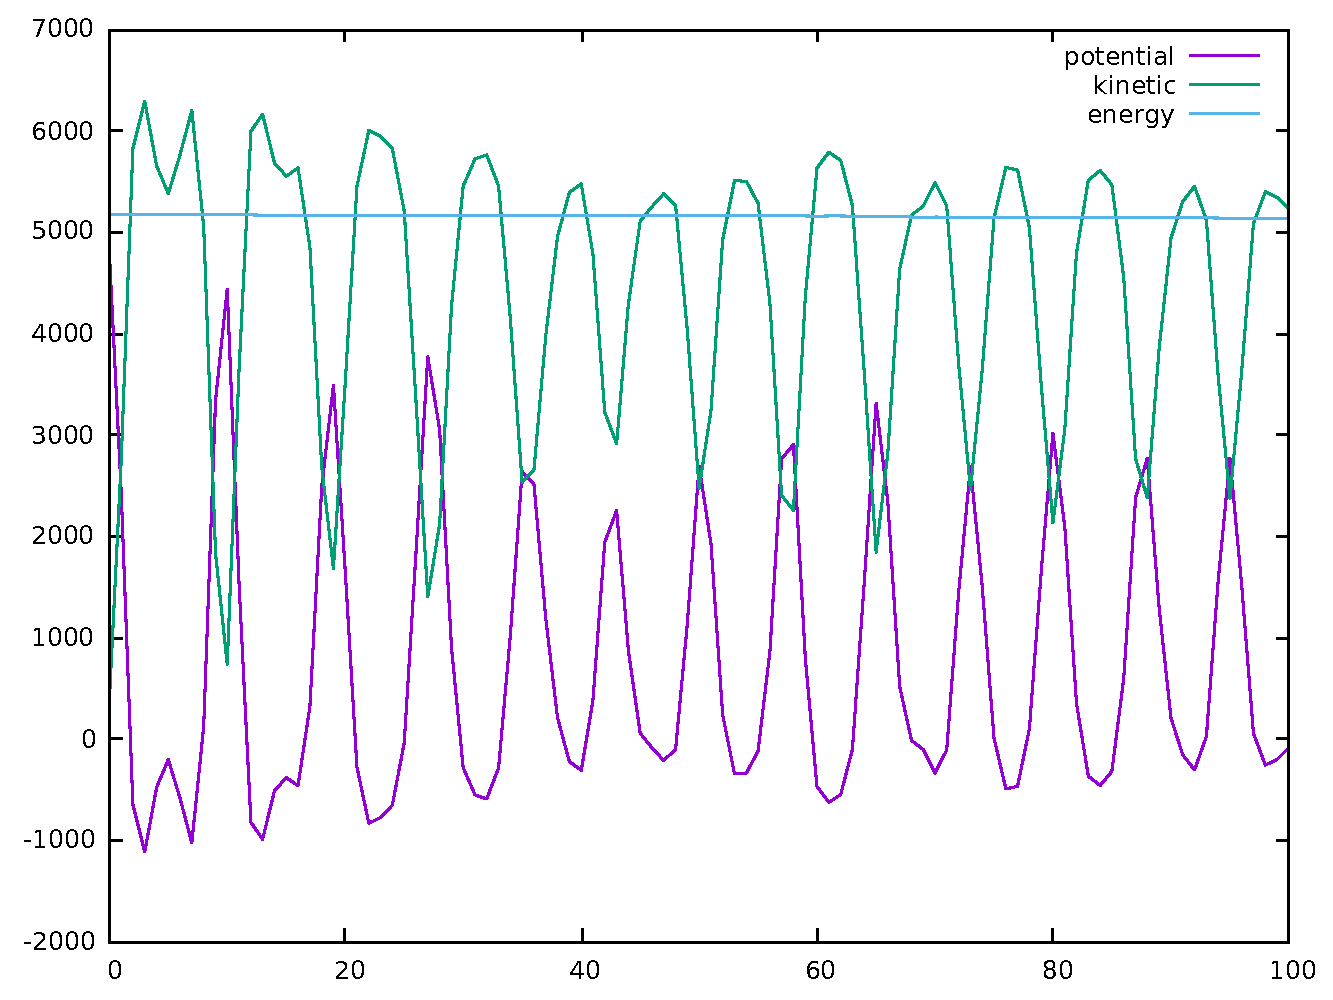
\includegraphics[width=1\linewidth]{env.pdf}
\caption{Action, kinetic term and Hamiltonian vs integration step; $(p,q)=(1,1)$; $n=20$; $g=-2.5$; $L=100$; $\tau = 0.0001$; time: 5s.}
\end{figure}

\newpage

\begin{figure}[hp]
\centering
\textbf{Energy violation in HMC, $10^3$ steps}
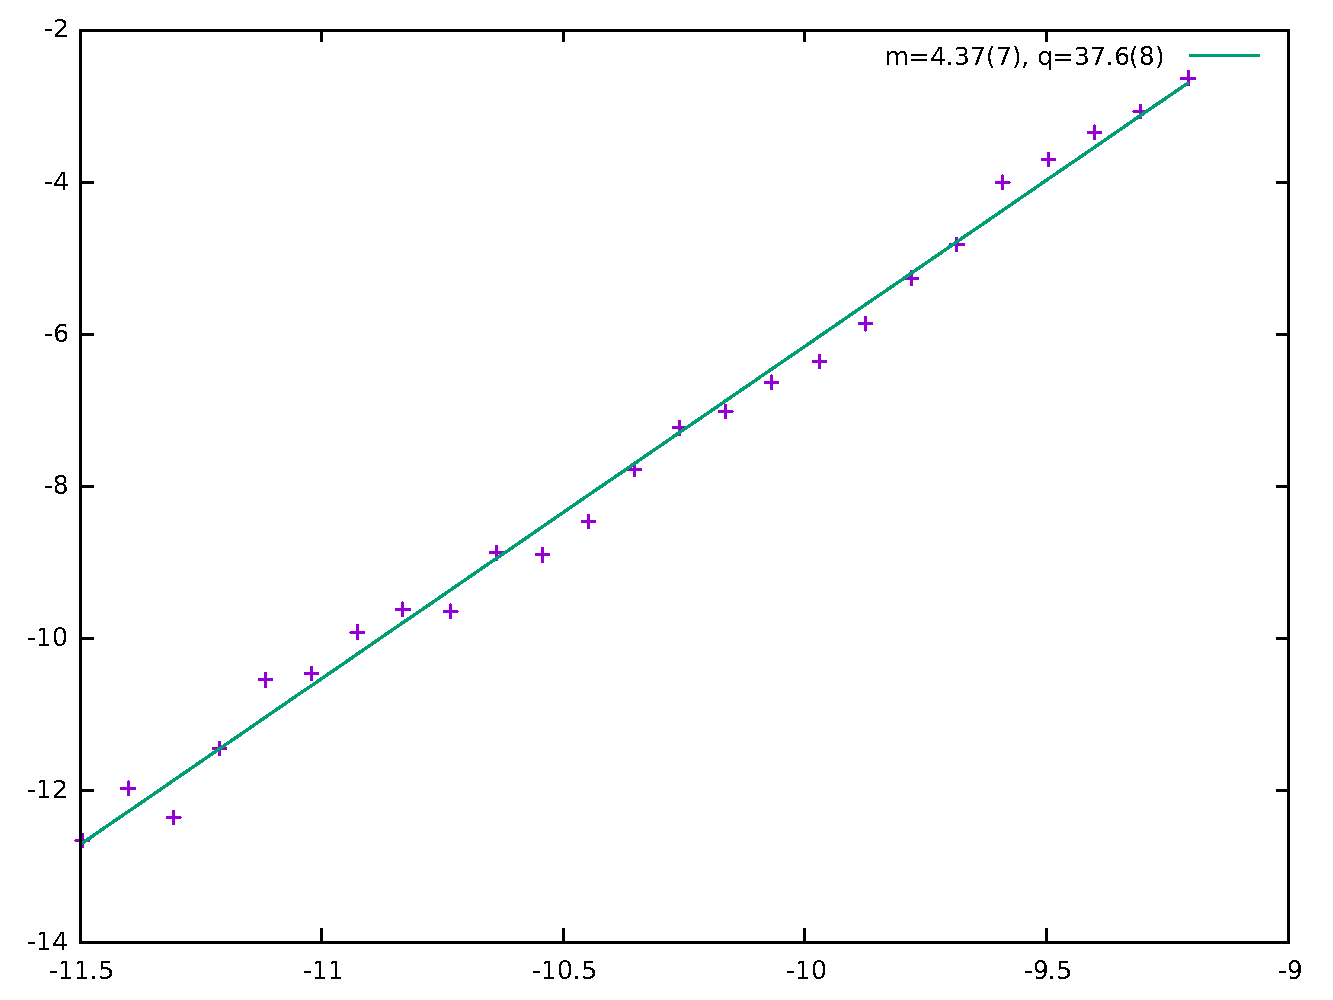
\includegraphics[width=1\linewidth]{quadratic103.pdf}
\caption{$\log \Delta H$ vs $\log \tau$ (purple): $(p,q)=(2,0)$; $n=10$; $g=-2.2431$; $L=10^3$; Linear fit (green): $m=4.37 \pm 0.07$, $q = 37.6 \pm 0.8$}
\end{figure}

\newpage

\begin{figure}[hp]
\centering
\textbf{Energy violation in HMC, $10^4$ steps}
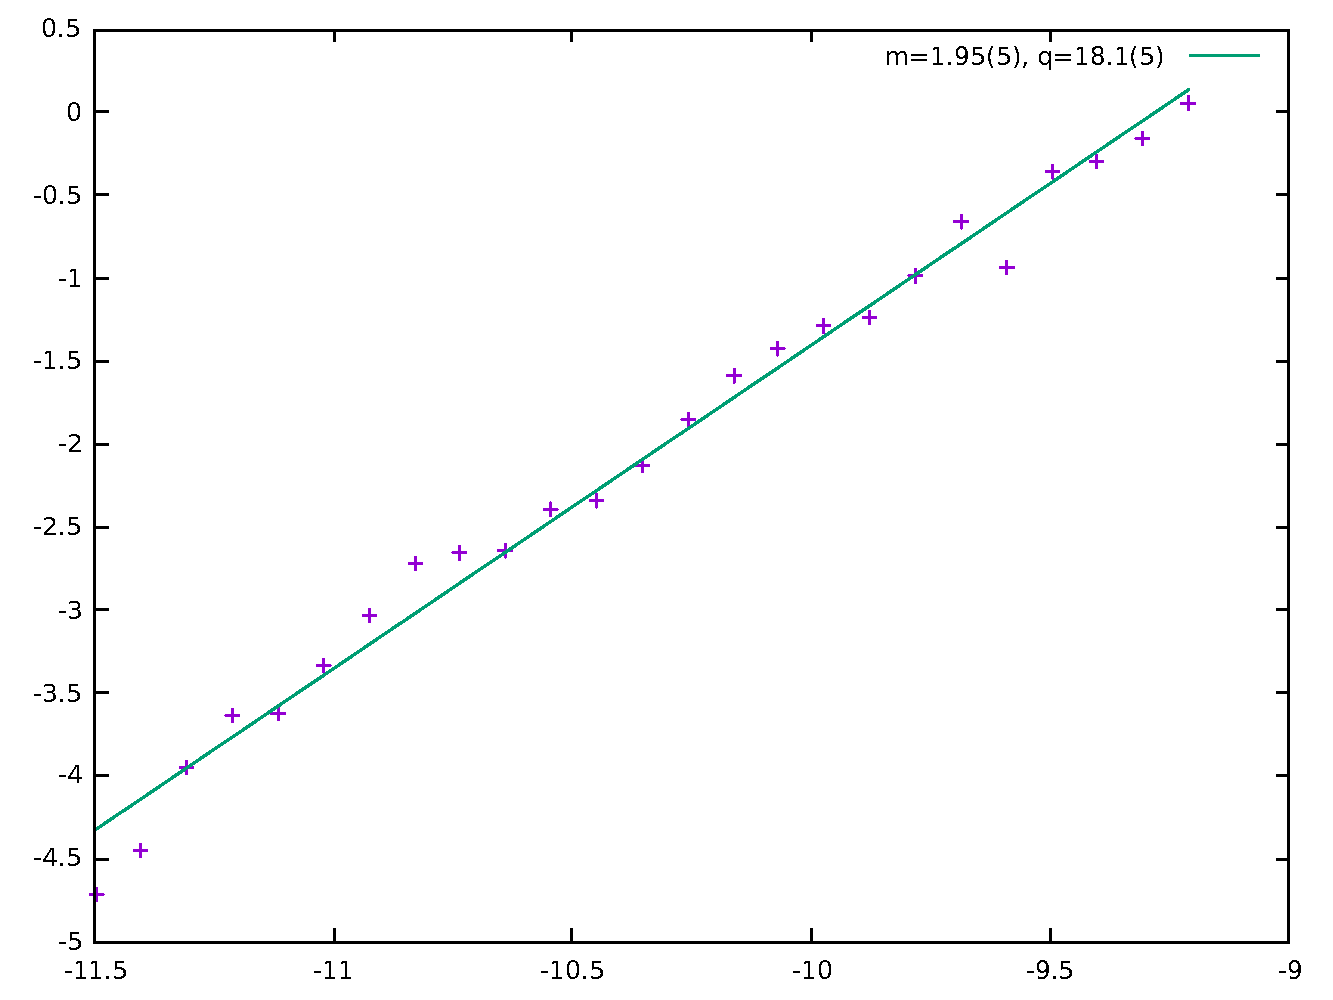
\includegraphics[width=1\linewidth]{quadratic104.pdf}
\caption{$\log \Delta H$ vs $\log \tau$ (purple): $(p,q)=(2,0)$; $n=10$; $g=-2.2431$; $L=10^4$; Linear fit (green): $m=1.95 \pm 0.05$, $q = 18.1 \pm 0.1$}
\end{figure}

\newpage

\begin{figure}[hp]
\centering
\textbf{Energy violation in HMC, $10^5$ steps}
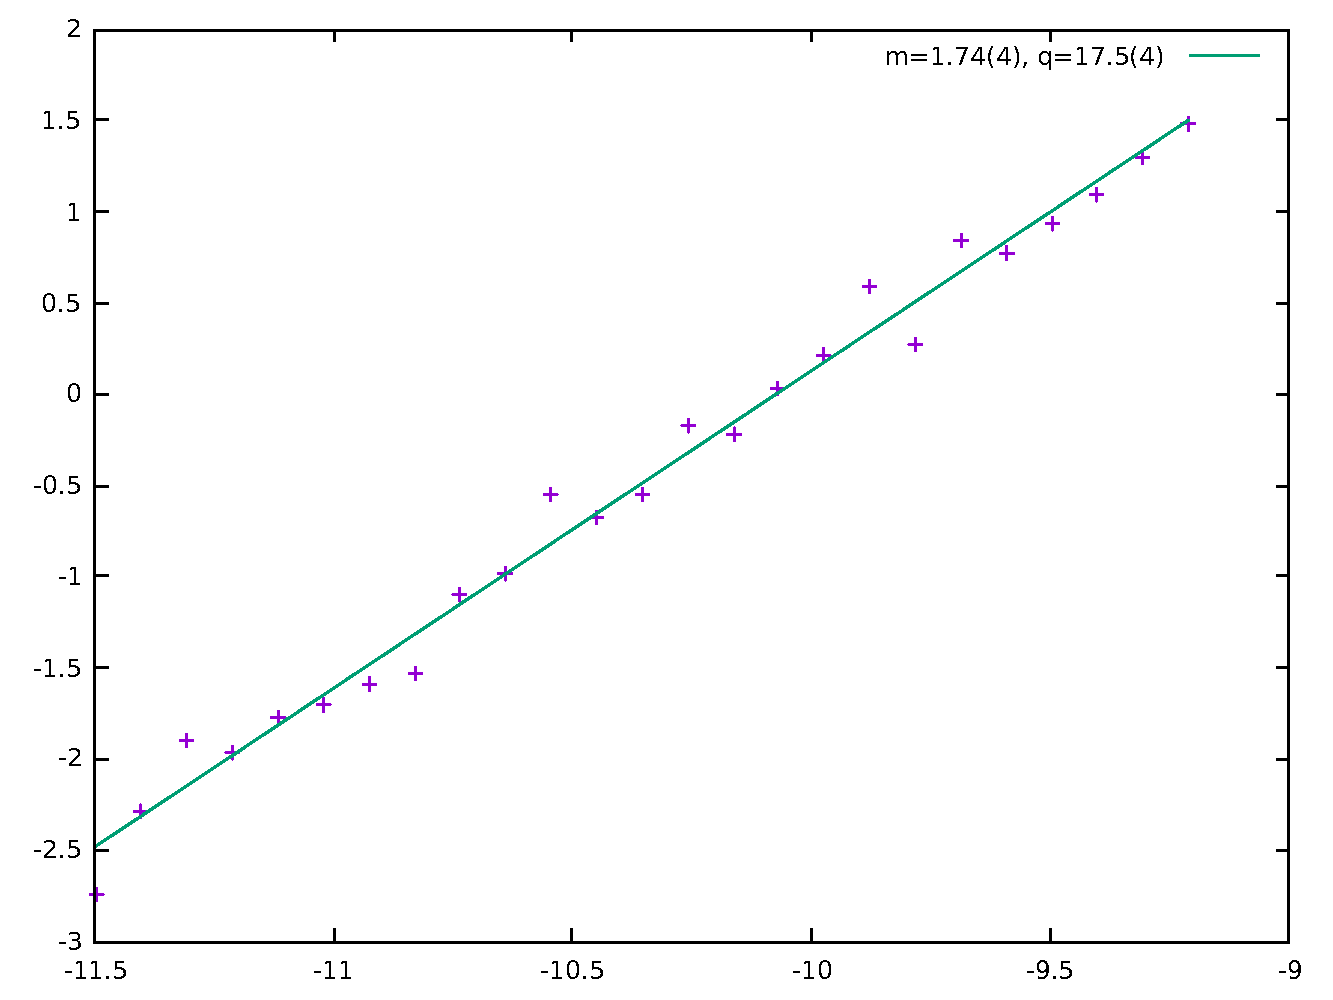
\includegraphics[width=1\linewidth]{quadratic105.pdf}
\caption{$\log \Delta H$ vs $\log \tau$ (purple): $(p,q)=(2,0)$; $n=10$; $g=-2.2431$; $L=10^5$; Linear fit (green): $m=1.74 \pm 0.04$, $q = 17.5 \pm 0.4$}
\end{figure}

\newpage

\begin{figure}[hp]
\centering
\textbf{Thermalization of $(1,1)$ geometry}
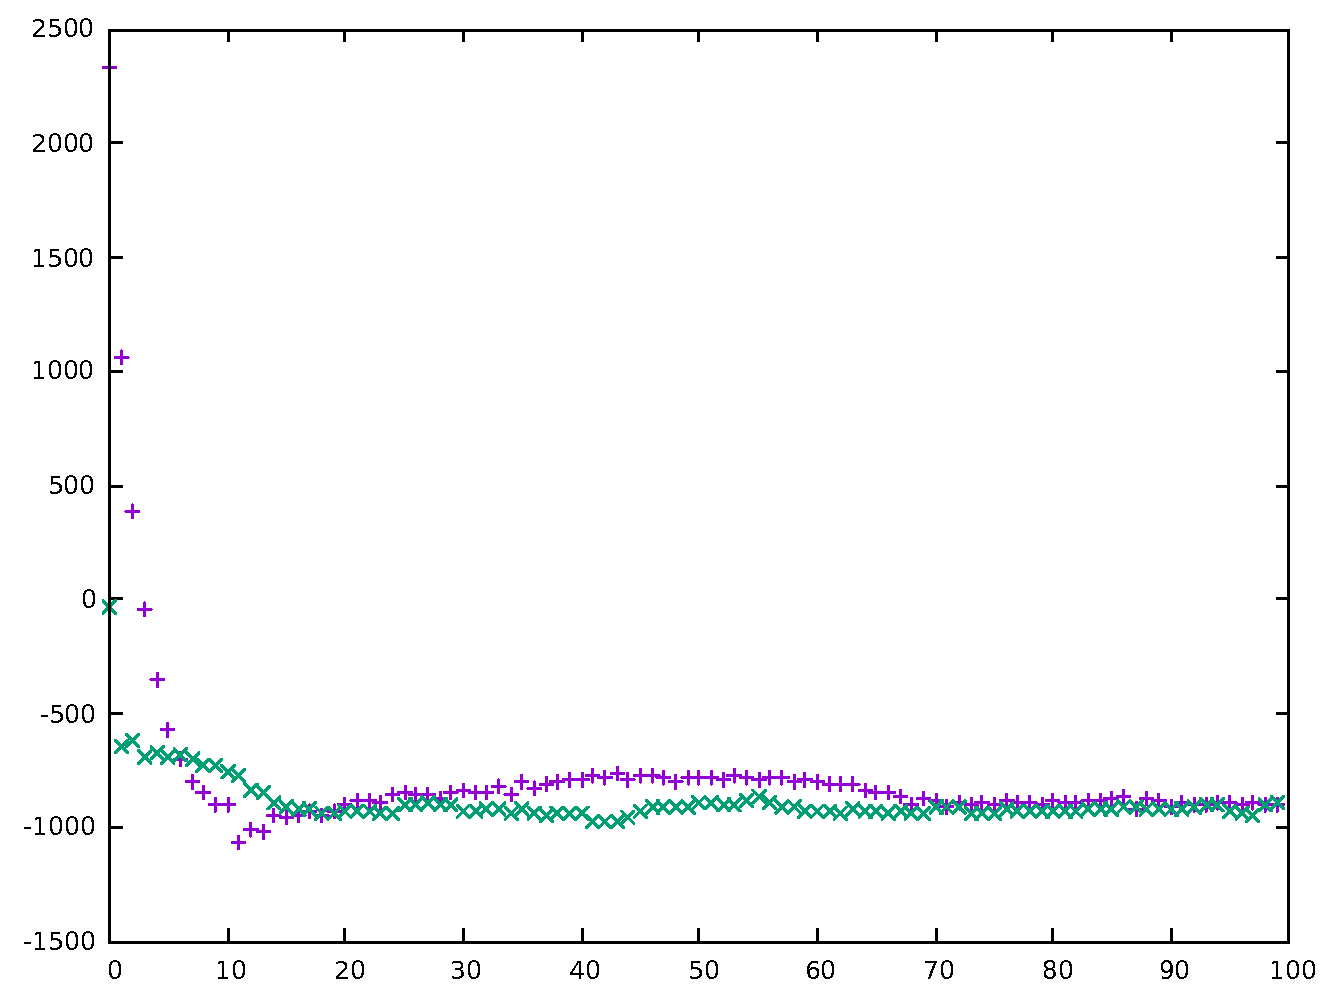
\includegraphics[width=1\linewidth]{p1q1n20g25.pdf}
\caption{Action $\Tr D^4 + g\Tr D^2$ vs Monte Carlo time; $(p,q)=(1,1)$; $n=20$; $g=-2.5$; $L=100$; $\tau_\text{cold10} = 0.0001$; $\tau_\text{cold90} = 0.0005$; $\tau_\text{hot} = 0.001$; time: 5s.}
\end{figure}

\newpage

\begin{figure}[hp]
\centering
\textbf{Thermalization of $(0,3)$ geometry}
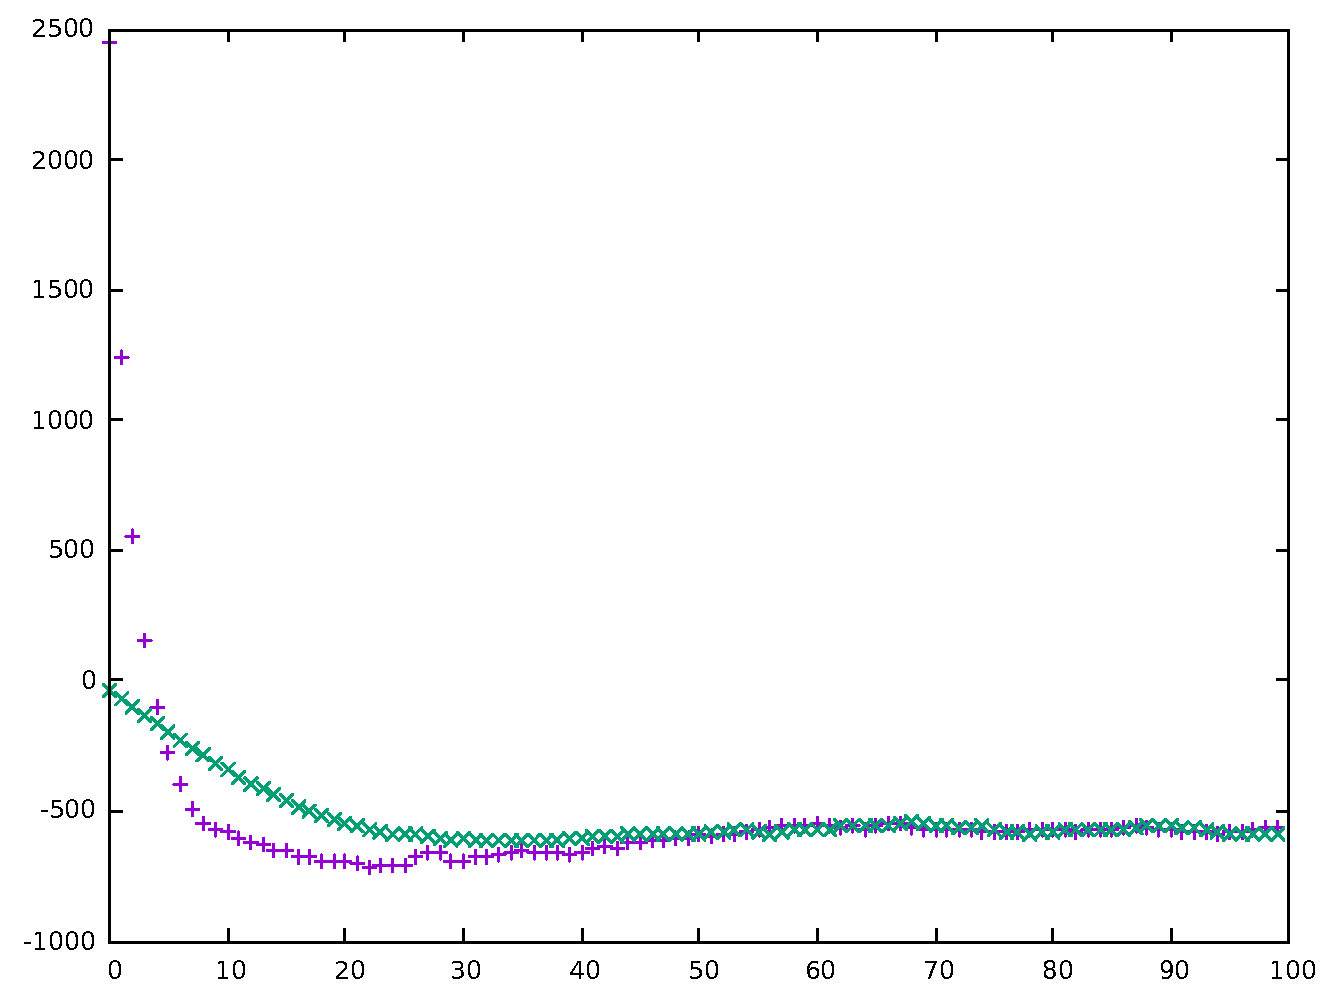
\includegraphics[width=1\linewidth]{p0q3n20g25.pdf}
\caption{Action $\Tr D^4 + g\Tr D^2$ vs Monte Carlo time; $(p,q)=(0,3)$; $n=20$; $g=-2.5$; $L=100$; $\tau = 0.0001$; time: 36s.}
\end{figure}

\newpage

\begin{figure}[hp]
\centering
\textbf{Thermalization of $(1,3)$ geometry}
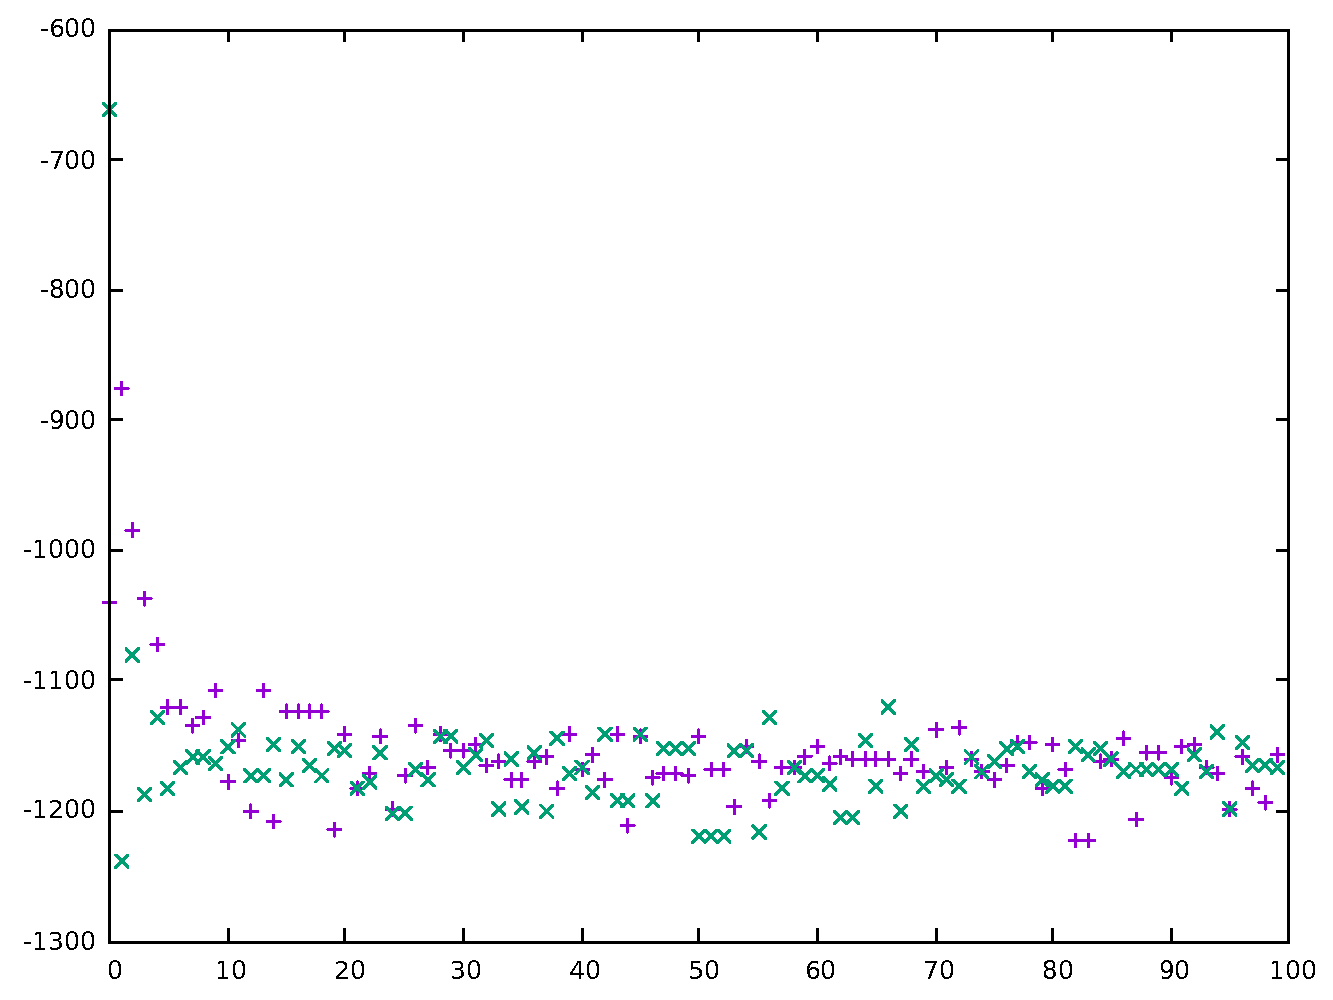
\includegraphics[width=1\linewidth]{p1q3n20g25.pdf}
\caption{Action $\Tr D^4 + g\Tr D^2$ vs Monte Carlo time; $(p,q)=(1,3)$; $n=20$; $g=-2.5$; $L=100$; $\tau_\text{cold10} = 0.001$; $\tau_\text{cold90} = 0.0005$; $\tau_\text{hot} = 0.0005$; time: 5m 40s.}
\end{figure}

\newpage

\begin{figure}[hp]
\centering
\textbf{Action $(2,0)$: comparison Metropolis/HMC}
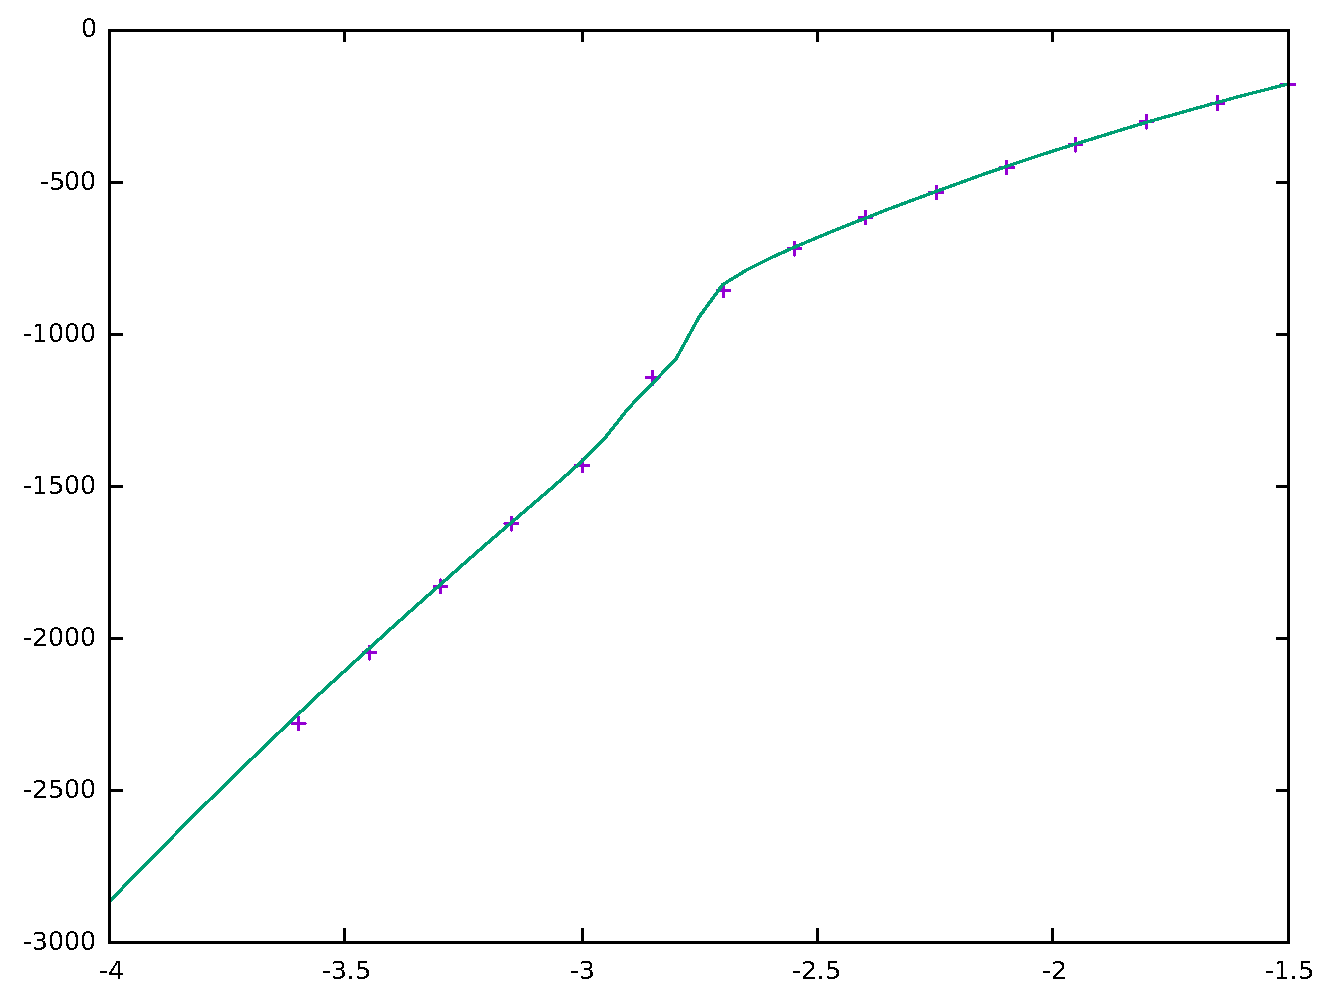
\includegraphics[width=1\linewidth]{p2q0n20S.pdf}
\caption{Action $\Tr D^4 + g\Tr D^2$ vs $g$; Metropolis (Green) and HMC (purple); $(p,q)=(2,0)$; $n=20$; $L=100$; $\tau = 0.0001$; time 13m 20s}
\end{figure}

\newpage

\begin{figure}[hp]
\centering
\textbf{Order parameter $(2,0)$: comparison Metropolis/HMC}
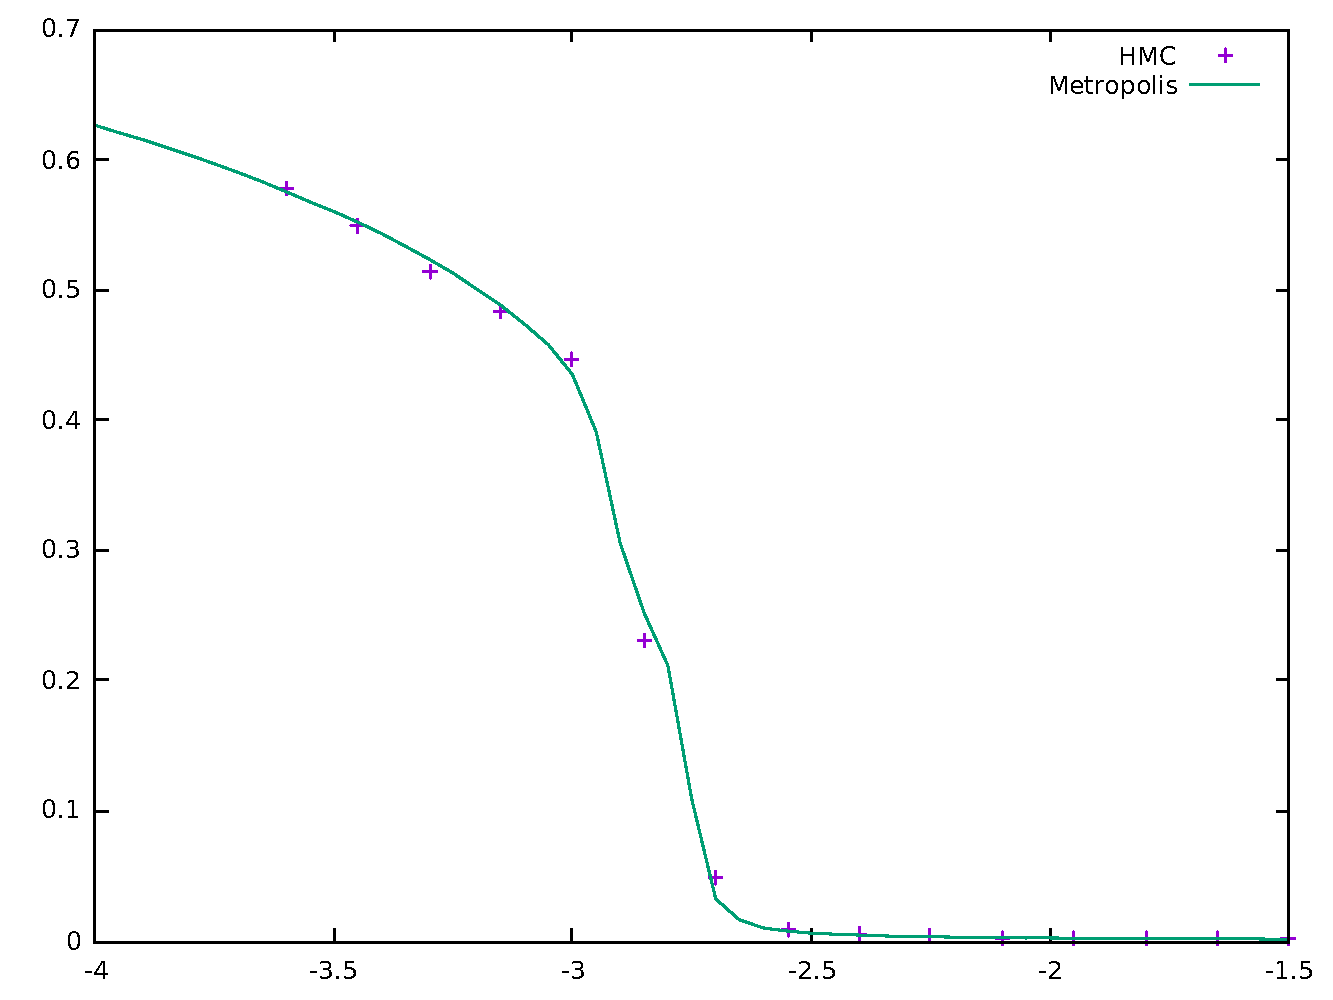
\includegraphics[width=1\linewidth]{p2q0n20F.pdf}
\caption{Order parameter vs $g$; Metropolis (Green) and HMC (purple); $(p,q)=(2,0)$; $n=20$; $L=100$; $\tau = 0.0001$; time 13m 20s}
\end{figure}

\newpage

\begin{figure}[hp]
\centering
\textbf{$\text{\# dofs} = 2 g_2 \langle S_2 \rangle + 4\langle S_4 \rangle$ test: comparison Metropolis/HMC}
\includegraphics[width=1\linewidth]{dofsp0q3.pdf}
\caption{Convergence of the expectation value of the observable $2 g_2 \Tr D^2 + 4 \Tr D^4 $ to the number of degrees of freedom of the Dirac operator for geometry $(0,3)$. The three sets correspond to matrix size $n = 16 \times 16$, $32 \times 32$ and $64 \times 64$. }
\end{figure}

\newpage

\begin{table}[hp]
\centering
\begin{tabular}{|l|l|l|}
\hline
\begin{tabular}[c]{@{}l@{}}Matrix\\ dimension\end{tabular} & \begin{tabular}[c]{@{}l@{}}time\\ HMC (sec)\end{tabular} & \begin{tabular}[c]{@{}l@{}}time\\ Metropolis (sec)\end{tabular} \\ \hline
16 & 23 & 17 \\ \hline
32 & 100 & 428 \\ \hline
64 & 1612 & 21218 \\ \hline
\end{tabular}
\caption{Time for 100 sweeps of HMC and Metropolis for geometry $(0,3)$. Fitting of the data gives a computational cost of $O(n^{4.6})$ and $O(n^{2.6})$ for Metropolis and HMC respectively.}
\label{tab:my-table}
\end{table}

\begin{figure}[hp]
\centering
\textbf{Autocorrelation of order parameter $(2,0)$ test: comparison Metropolis/HMC}
\includegraphics[width=1\linewidth]{autocorrp2q0.pdf}
\caption{Autocorrelation $\chi (a) = \langle F(t)F(t+a) \rangle - \langle F(t) \rangle \langle F(t+a) \rangle$ normalized by $\chi(0)$, where $F(t)$ is the order parameter for the $(2,0)$ phase transition at Monte Carlo time $t$. The coupling constant $g_2 = 2.725$ was chosen to be at the phase transition. The exponential fit gives an autocorrelation time of $\sim 250$ sweeps for Metropolis and $\sim 25$ sweeps for HMC.}
\end{figure}








\end{document}
